\section{Analysis Overview}
\label{sec:analysis_overview}
The first step to performing a precision measurement of the Higgs boson mass (\mH) is to ``observe'' many Higgs bosons.
However, production of a Higgs boson is essentially nonexistent in everyday conditions and is still extremely rare even in the high-energy \pp collisions of the LHC.
At a center-of-mass energy of 13\TeV, the total inclusive inelastic cross section of two protons colliding is 70\mb TODO: CITE.
Comparing this to the production cross section of a Higgs boson (TODO sigma(pptoH) = 59 pb) shows that a Higgs boson is produced in approximately one out of every billion \pp collisions.  TODO CITE

To complicate matters further, the Higgs boson has a \emph{very} short mean lifetime of only $1.6 \tentotheminus{22}\snd$~\cite{pdg}.
Thus, the Higgs boson is not directly detected by CMS but is instead \emph{inferred} from its stable decay products that enter the various subdetectors.
Among all the fundamental particles so far discovered, the Higgs boson bears the second heaviest mass (approximately 125\GeV), the first belonging to the top quark (Section~\ref{sec:sm}).
This gives the scalar boson sufficient energy to decay into at least 9 different final states.
\textcolor{red}{MENTION THAT NOT ALL DECAYS MAKE ON-SHELL PARTICLES?}
Each decay occurs with a different probability---the \emph{branching fraction} or \emph{branching ratio} (\br)---whose value depends on \mH as shown in Figure~\ref{fig:higgs_br}.
\begin{figure}[!htbp]
    \begin{center}
        % Figures come from:
        % https://twiki.cern.ch/twiki/bin/view/LHCPhysics/LHCHWG?redirectedfrom=LHCPhysics.LHCHXSWG#Higgs_cross_sections_and_decay_b
		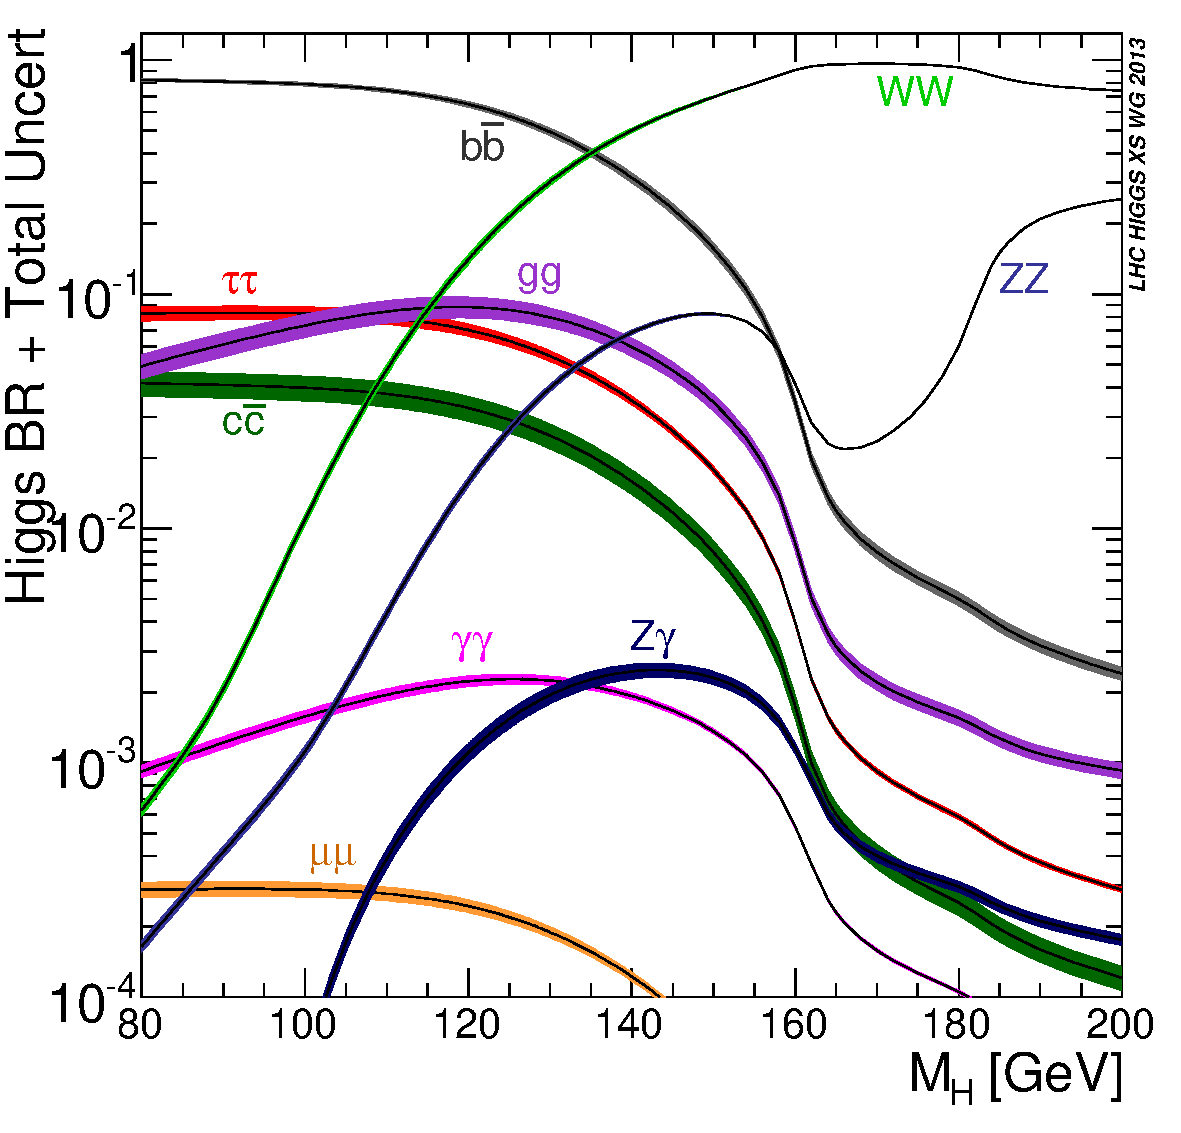
\includegraphics[width=0.48\textwidth]{figures/higgsmassmeas/higgs_BR_80to200GeV.pdf}
		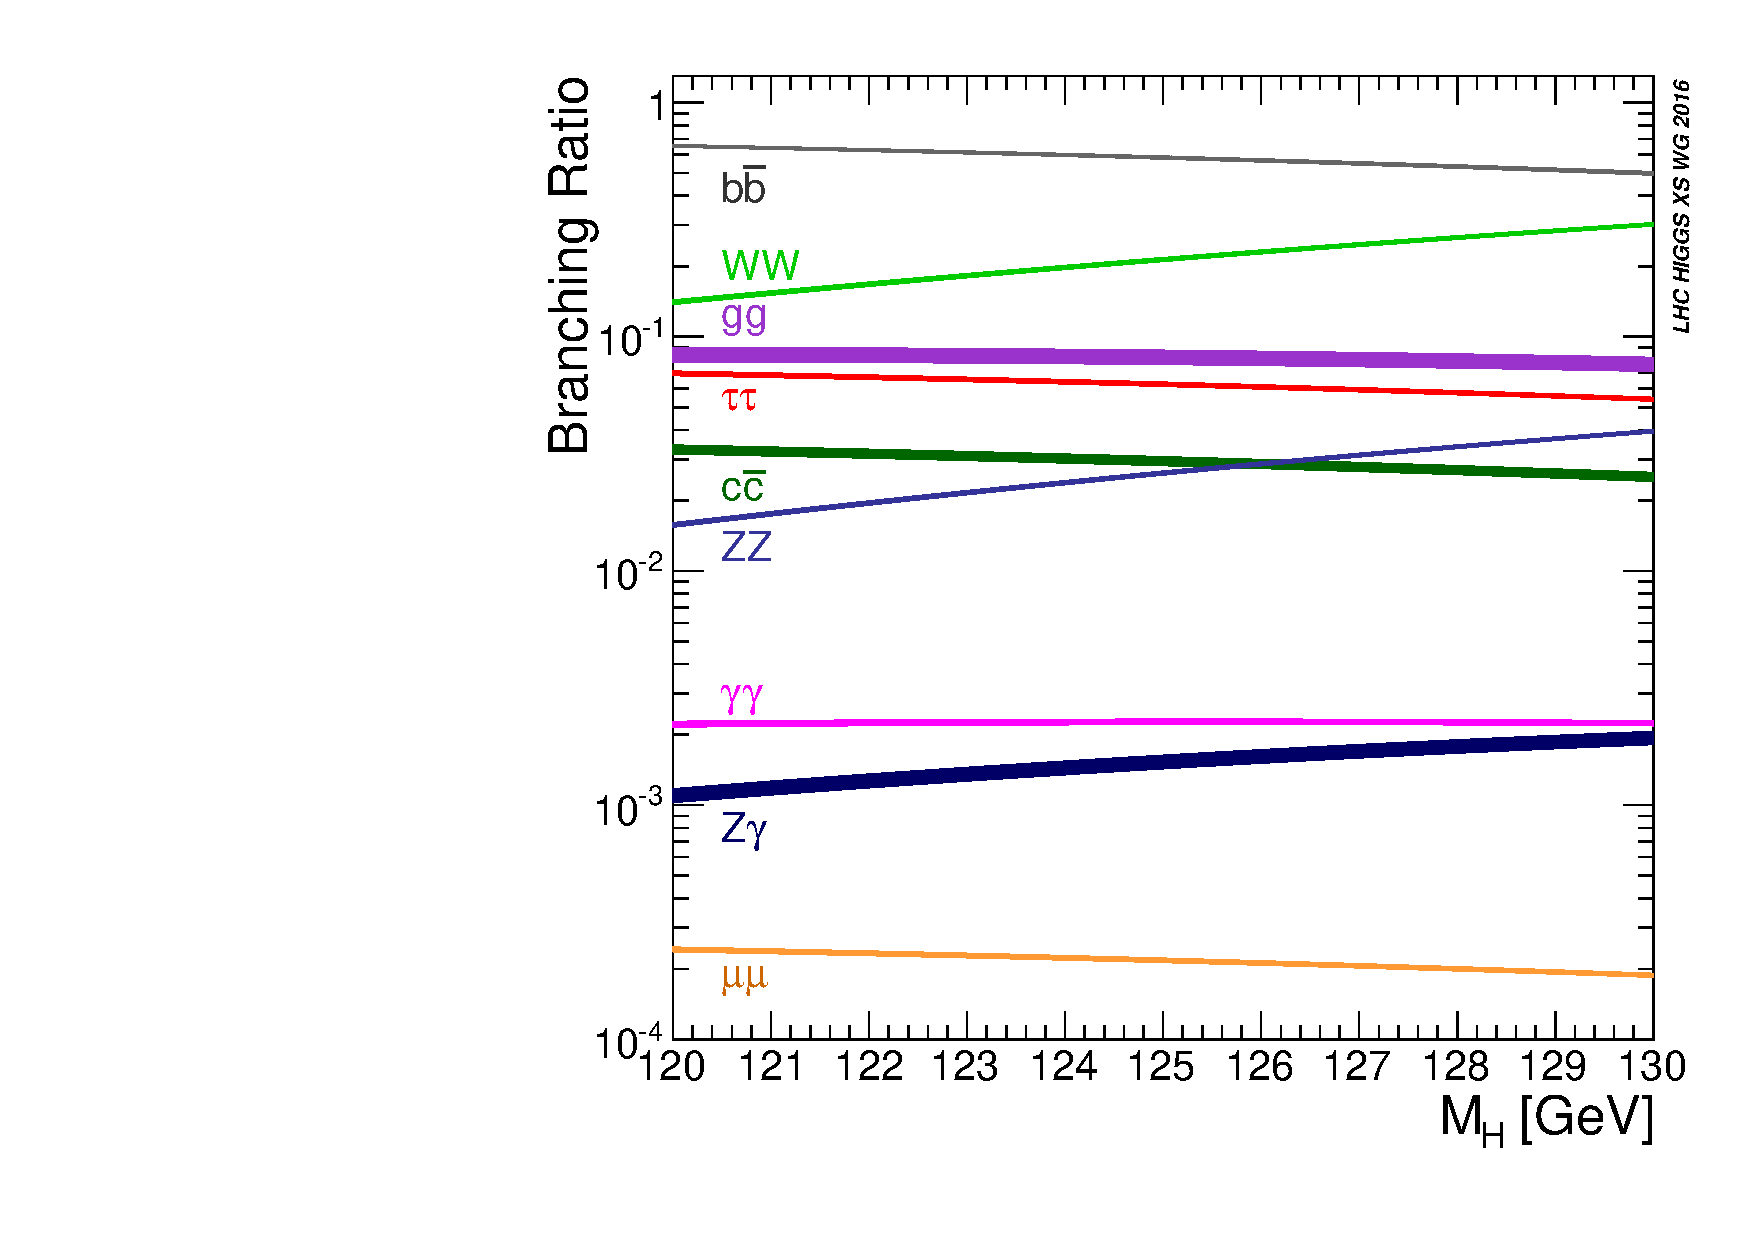
\includegraphics[width=0.48\textwidth]{figures/higgsmassmeas/higgs_BR_120to130GeV.pdf}
		\caption{
            The branching ratios of various Higgs boson decays as a function of the Higgs boson mass
            over a wide range of values (Left) and a narrow range (Right).
            }
		\label{fig:higgs_br}
	\end{center}
\end{figure} 
The question then becomes, \emph{``Which decay mode of the Higgs boson is most useful for the measurement of \mH?''}.
Owing to its large signal-to-background ratio of approximately 2 and its relatively rare four-lepton final state, the \hzzfourl decay channel is selected and is called the \emph{signal} process.
Thus, a single Higgs boson decays via the signal process into two \PZ bosons (one on-shell and one off-shell) only 2.6\% of the time.
In turn, each \PZ boson decays into two opposite-sign, same flavor (OSSF) leptons (\Ztolplm, where $\ell = \Pe, \mu$) on average approximately 6.7\% of the time, giving rise to four distinct final states:
\foure, \fourmu, \twoetwomu, \twomutwoe.
The branching ratio for the overall signal process is then calculated as: % B(Z->ee)=0.033632, B(Z->mumu)=0.033662
\begin{equation*}
    \BRof{\hzzfourl} = \BRof{\htozz} \left[ \BRof{\Ztolplm} \right]^2 = 1.8\tentotheminus{3}.
\end{equation*}
Thus, a signal event is expected to be produced only once in about every \emph{trillion} \pp collisions.

The strategy is then to search the \pp collision data collected and analyzed by the CMS detector (Chapter~\ref{ch:cms_detector}) for all the detected \hzzfourl events.
The task is not so straightforward;
events in the data are categorized---not by the entire decay process---but by their final state, based on which triggers fired to collect which events.
Section~\ref{sec:datasets_simul_trig} describes the triggers used for this analysis to select events with the \fourl final state found in the corresponding data sets.
The chosen events have a plethora of information from all the various subdetectors in CMS (Chapter~\ref{ch:cms_detector}) which gets reconstructed into \emph{objects}---representations of the true particles produced by the event.
Since the process of interest is \hzzfourl, the reconstructed objects per event should be assembled in a fashion that coincides with the  of each event should resemble this process, 
The reconstructed objects per event must then be assembled in a fashion that coincides with the logic of the process of interest: \hzzfourl.
So, for example, two OSSF-dilepton objects should each appear to come from a \PZ-boson-like object (\eg having a nominal mass of approximately 91\GeV and zero net electric charge)---instead of, say, coming from a Higgs-boson-like object.
Furthermore, the involved objects should obey physics conservation laws (energy, momentum, charge, \etc) and pass detector selection criteria.
These requirements are analysis-specific \emph{event selection} process to ensure that the events 

Once all signal-like events have been identified...

BACKGROUND

by being combined in a specific fashion and be combined in such a way so as to resemble this process, \eg 

% Real particles enter detectors in CMS which send signals to various electronics.
% Particle Flow algorithm pieces the information together to construct objects out of each event.
% Now, instead of just a deposit of energy in the ECAL and corresponding hits in the silicon tracker, the particle is identified as a newly produced electron.
% CMS records which kinds of objects came from which events and stores the information in \emph{data sets} (TODO: ref Section future).

BACKGROUND
- By collecting events with the \fourl final state, we are likely to find signal events.
    - It's not just the signal process which produces \fourl: background also makes \fourl (Section FIXME).

- Before analyzing the data, however, it is important to make predictions using simulated samples (Section FIXME).
- In order to sort signal from background, use simulated samples 

, which is the formation of particle physics objects from data.
The data collected and analyzed by CMS is not so simple so as to have \htozz

This process hinges on the conservation of momentum, since in the longitudinal ($z$) direction the \pp collision has initial and final.
Specifically, the 
    - The \PZ boson has a precisely measured mass of TODO a neutral particle, so the two leptons into which it decays should combine to Group two leptons together, 
    - Form two different pairs of opposite-sign, same-flavor (OSSF) leptons
    - If it appears that the to select specific hzz4l events (\emph{event selection}).